% !TeX root = ../main.tex
% INDEPENDENT TASK MODULE. Comment out its single \input line in main.tex to remove it.
\clearpage
\chapter{Task \#39 -- \textbf{Epidemic spreading on cruise-ship temporal contact networks}}\label{chap:cruise-epidemic}

\section{Introduction}

This project uses cruise ship contact data to investigate how the timing and structure of human interactions affect disease spreading. It compares the empirical time-varying network with its static aggregation and with two randomized surrogate networks, to determine whether neglecting chronological order or empirical contact structure inflates or reduces the predicted size of an outbreak.

Data come from the public repository associated with Pung \emph{et al.}~\citep{pungCruiseNetworks}. The two primary files are \texttt{dataNodes.RData}, which contains individual-level node metadata, and \texttt{dataContact.RData}, which contains contact episodes between pairs of individuals. This analysis uses sail 1 only, for which contacts are observed over three days. 
We export those data to CSV and construct three processed files: \texttt{nodes\_sail\_1.csv}, containing nodes IDs and additional metadata; \texttt{temporal\_edges\_sail\_1.csv}, 
containing contacts happening all over the three observed ddays with cumulative contact duration; and \texttt{aggregated\_edges\_sail\_1.csv}, a static edge list whose weights are total contact durations.\\
Four network representations are used for the analysis. The \emph{empirical temporal} network preserves the observed interaction day of each pair and uses cumulative pair duration within that day as edge weight. 
The \emph{aggregated static} network is constructed by aggregating all time-ordered interactions into permanent and simultaneous connections, where the weight of each edge is the total contact duration between the two individuals, divided by the total number of observed days.
Two surrogate networks are also used as null models: the \emph{temporal Erd\H{o}s--R\'enyi (ER)} network considers the daily empirical edges and preserves the exact number of connections
 and their weights at each temporal step, but randomly shuffles the interacting nodes; the \emph{static ER} network preserves the number of nodes and edges in the aggregated network, but completely randomizes the connections between nodes and randomly shuffles the existing contact weights among the newly created edges.
The reconstructed population (see appendix table~\ref{tab:cruise-network-characteristics} for the details) contains therefore $N=2240$ individuals, $E=357\,656$ total temporal contacts among the three days and $E=309\,139$ edges in the aggregated static graph. The aggregated network merges repeated contacts between any pair of individual among the three 
days into a single permanent edge, resulting in a lower count of total edges.

\begin{figure}[H]
\centering
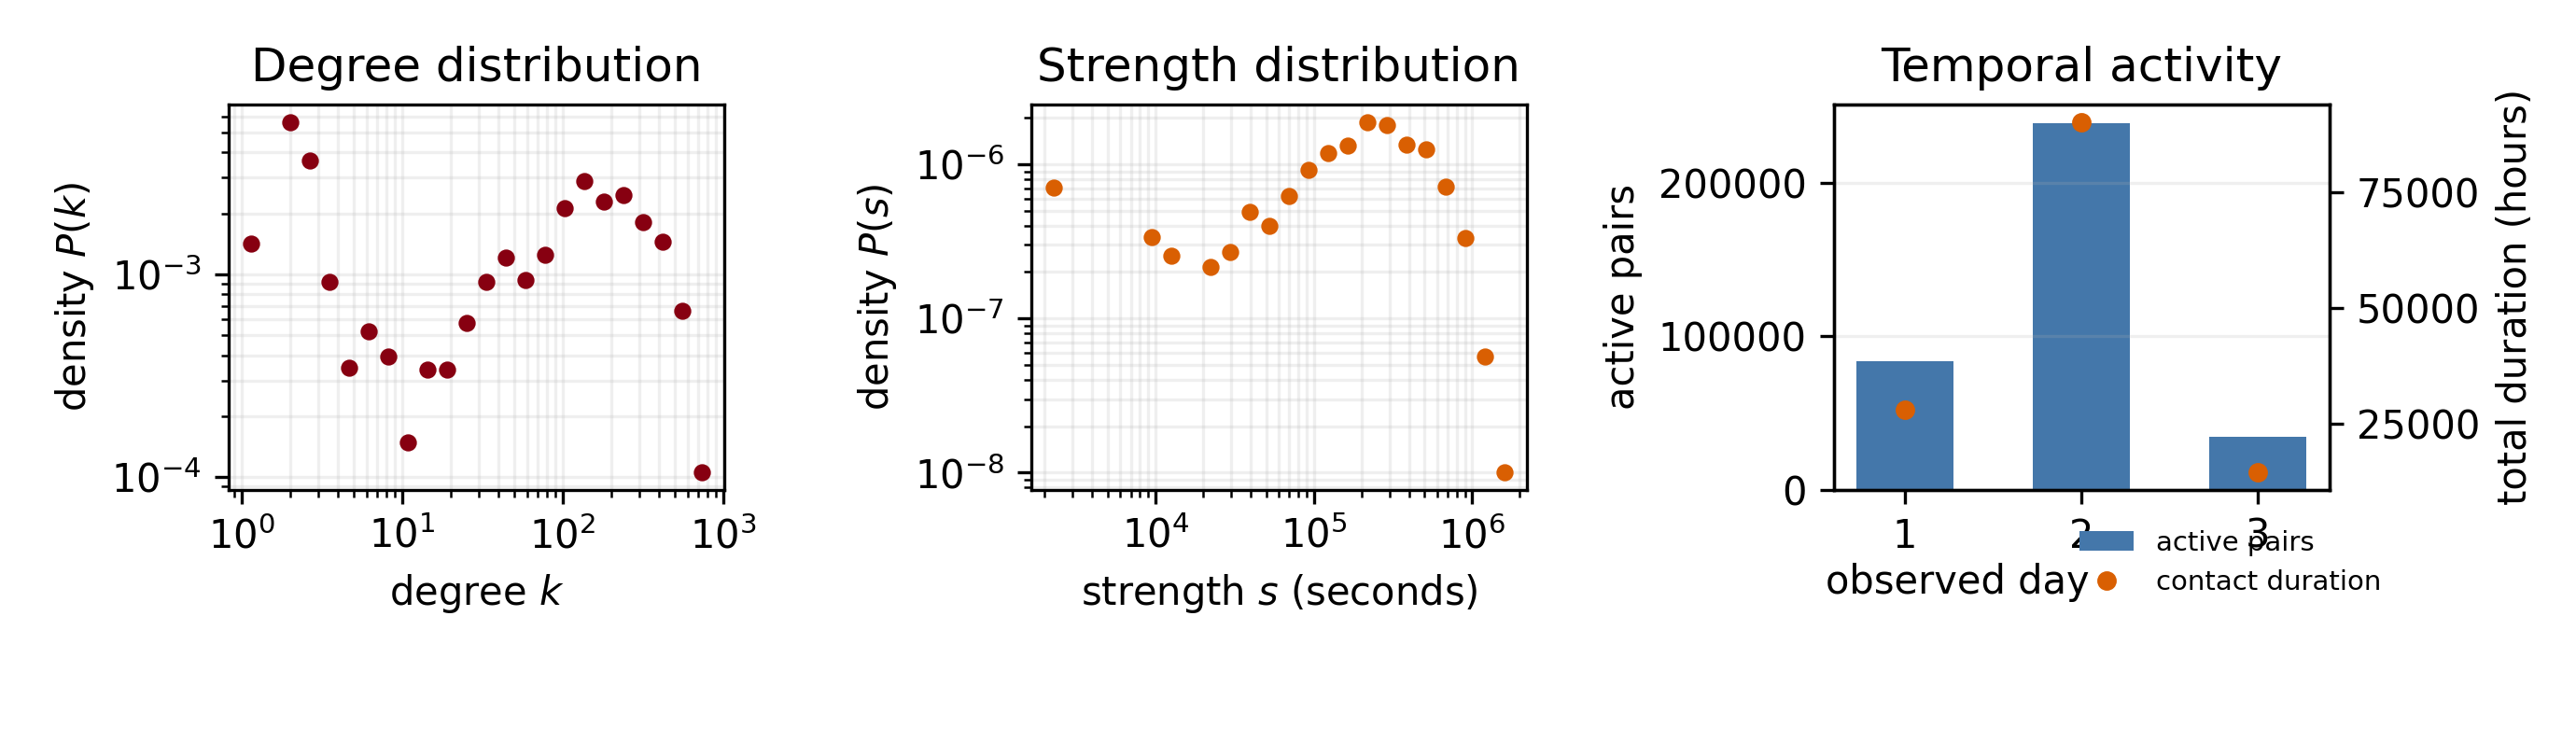
\includegraphics[width=.96\linewidth]{results/cruise_epidemic_corrected/empirical_network_descriptives.png}
\caption{Descriptive properties of the empirical sail-1 data. Degree and strength are computed on the aggregated empirical graph; strength is the total contact duration accumulated over the three observed days. The temporal-activity panel shows the number of active pairs and the total contact duration in each daily snapshot.}
\label{fig:cruise-descriptives}
\end{figure}

\section{Epidemic model}

The simulation uses a stochastic discrete-time SEIR process. Individuals are in four possible states: susceptible ($S$), exposed ($E$), infectious ($I$), or recovered ($R$). At each time step, infectious individuals can infect susceptible neighbours along the currently active edges. For an edge with duration or weight $w_{uv}$, the infection probability is
\[
p_{uv}=1-\exp\!\left(-\beta\frac{w_{uv}}{1800}\right)
\]
where $w_{uv}$ is contact duration in seconds and $1800$ is the default half-hour scale. Exposed individuals become infectious with probability $\sigma$ per day, and infectious individuals recover with probability $\gamma$ per day. 
The default values are $\sigma=0.5$ and $\gamma=1/3$. Since empirical data cover three observed days, the simulation cycles the temporal pattern over a total of $21$ days.

The order parameter is the mean attack rate , which is the final fraction of individuals that have left the susceptible state, as function of the transmission probability $\beta$. In a single stochastic realization $r$ it is given by
\[
A_r(\beta)=\frac{N_E(T)+N_I(T)+N_R(T)}{N}=1-\frac{N_S(T)}{N},
\]
where $T$ is the final simulated day. For $R$ realizations, the reported order parameter is $\overline{A}(\beta)=R^{-1}\sum_{r=1}^{R}A_r(\beta)$.


\section{Simulation results}

For each $\beta\in\{0.02,0.05,0.08,0.12,0.16,0.22,0.30,0.40\}$, the reported mean attack rate is estimated from $1000$ independent stochastic realizations. 
Fig.~\ref{fig:cruise-results} shows that the aggregated static representation systematically gives larger mean attack rates than the empirical temporal network, especially for low $\beta$ values. 
This overestimation decreases for large $\beta$ and the reason is that, when $\beta \to 1$, almost every contact leads to transmission, therefore after 21 days of simulation all the networks should exhibit an attack rate close to $1$. Instead, at intermediate \(\beta\) values, chronology of contacts matters much more and leads to differences in the results.
The ER surrogate network show even stronger overestimations for all $\beta$ values. In fact, temporal ER shuffles the contact pairs and thus removes correlations between who meets whom, resulting in an epidemic that reaches different groups more efficiently. 
On the other hand, static ER randomizes the topology as well, but it also makes contacts permanently available, producing the largest outbreaks of the epidemic.  \\
The conclusion is that, for this cruise population, replacing the specific temporal sequence of contacts with links that are permanently available inflates final epidemic size, particularly at moderate transmission.
The comparison of the surrogate ER networks with the empirical representations
shows that the larger outbreaks on both ER networks indicate that the observed
organization of contacts, and not only their number and duration, limits
epidemic spreading.
\begin{figure}
\centering
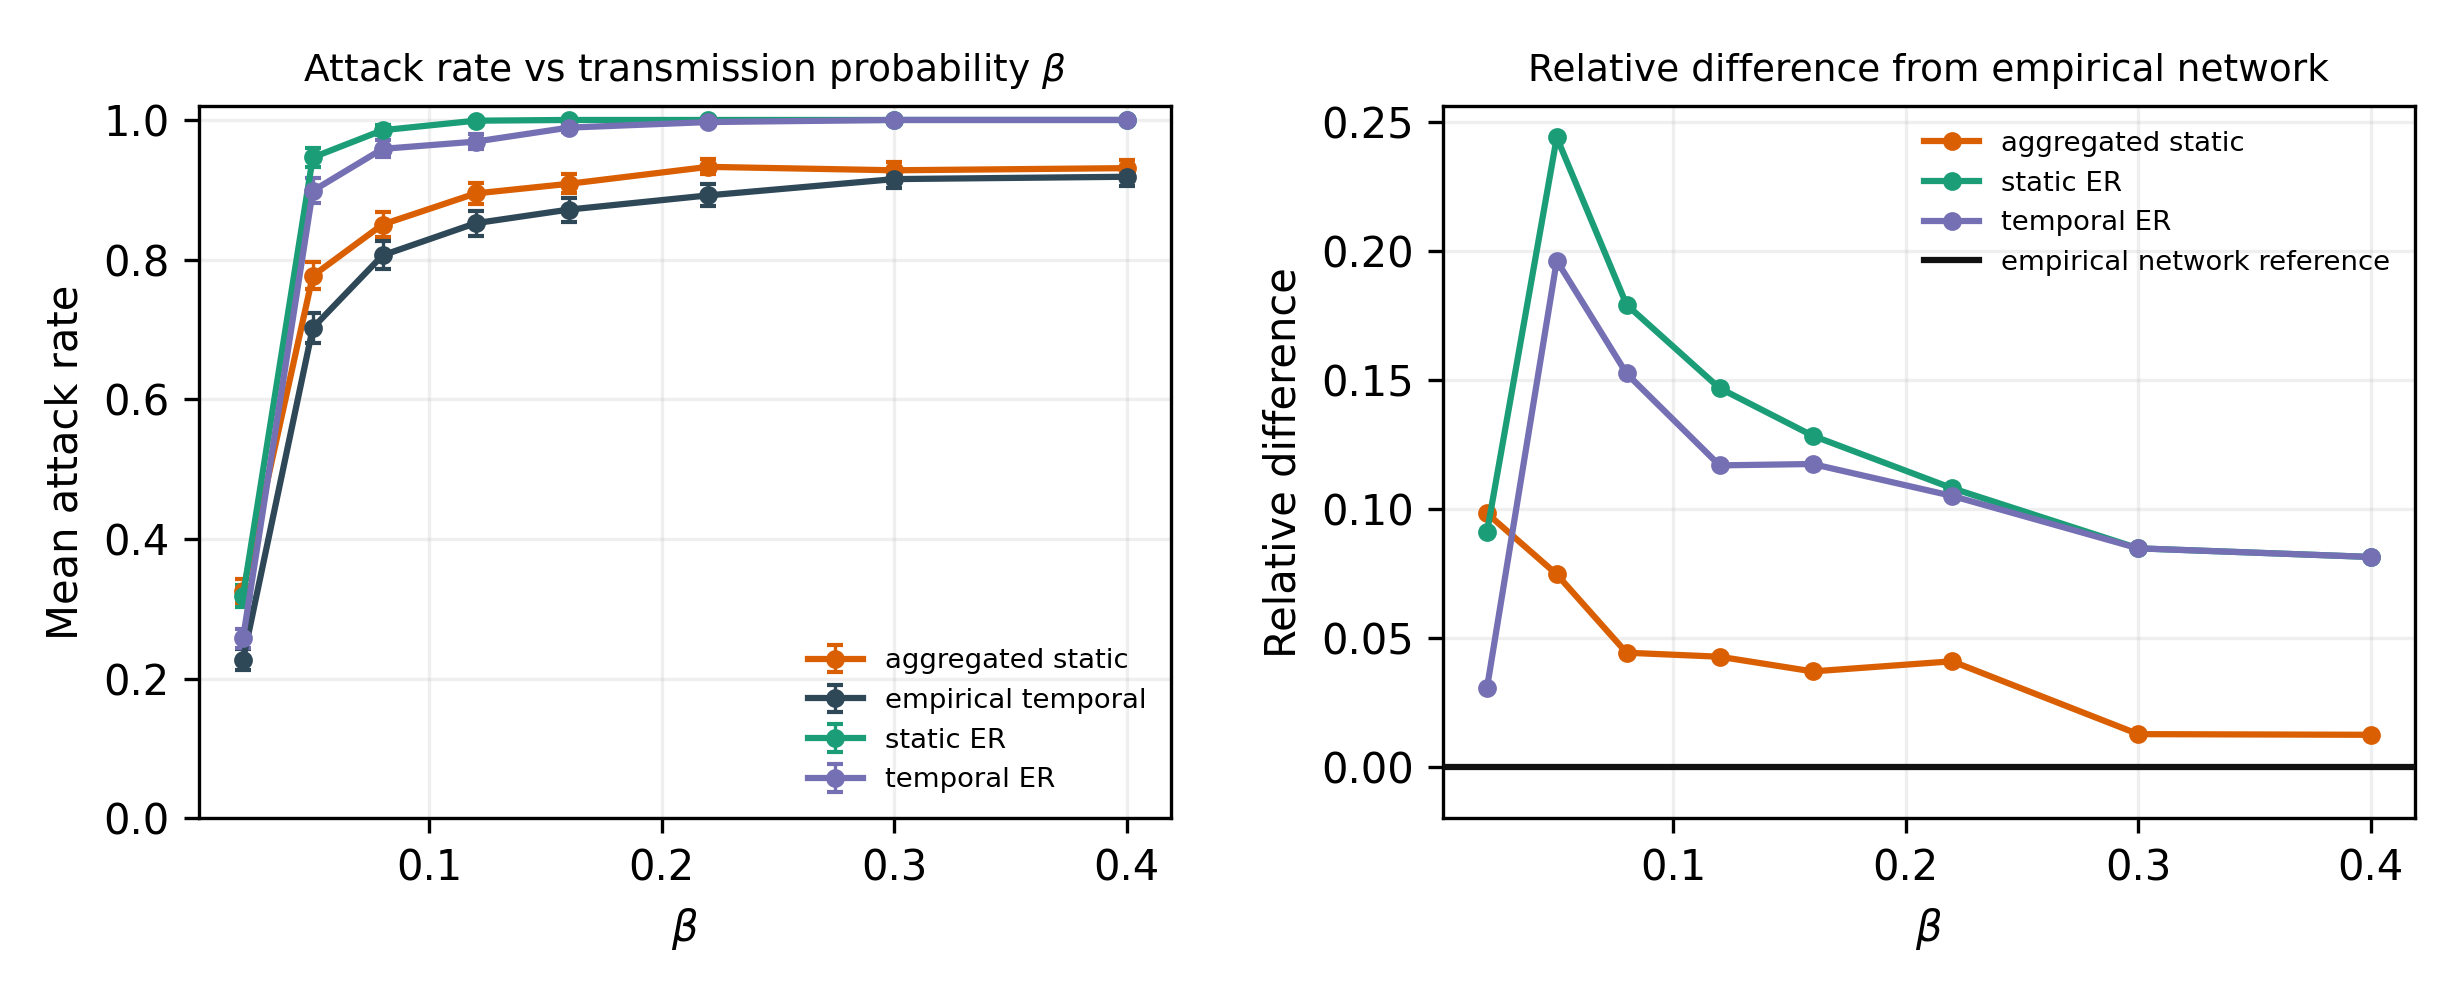
\includegraphics[width=.96\linewidth]{results/cruise_epidemic_corrected/corrected_temporal_comparison.png}
\caption{SEIR results for the four network representations. Left panel: mean attack rate as function of the transmission probability $\beta$ across the four different network representations. Right panel: relative difference between each network attack rate and the empirical temporal network attack rate. The horizontal black thick line refers to the temporal network reference.}
\label{fig:cruise-results}
\end{figure}




\clearpage
\section*{Appendix: Network characteristics and seed-node dependence optional extension}
\addcontentsline{toc}{section}{Appendix: Network characteristics and seed-node dependence}

\begin{table}[H]
\centering
\scriptsize
\renewcommand{\arraystretch}{1.08}
\setlength{\tabcolsep}{3.5pt}
\begin{tabular}{lccccc}
\toprule
Representation & Nodes & Edges & \shortstack{Mean\\degree} & \shortstack{Average local\\clustering $\overline{C}$} & \shortstack{Degree\\assortativity $r$} \\
\midrule
Empirical temporal & $2240$ & $(83\,759,\,239\,279,\,34\,618)$ & $(74.8,\,213.6,\,30.9)$ & $0.274$ & $0.154$ \\
Aggregated static & $2240$ & $309\,139$ & $276.02$ & $0.321$ & $0.191$ \\
Temporal ER & $2240$ & $(83\,759,\,239\,279,\,34\,618)$ & $(74.8,\,213.6,\,30.9)$ & $0.048$ & $-0.003$ \\
Static ER & $2240$ & $309\,139$ & $276.02$ & $0.123$ & $-0.001$ \\
\bottomrule
\end{tabular}
\caption{Network characteristics used in the simulations. For temporal networks, clustering and assortativity are averaged across the three daily snapshots; for static networks, their values are computed on the single static graph. Both metrics use the unweighted topology. This means that, for example, the clustering just counts the number of triangles without considering the duration of the contacts.}
\label{tab:cruise-network-characteristics}
\end{table}

\subsection*{Dependence on the initial seed node}

The seed-node experiment samples the initial infectious node uniformly from one of five pools: all nodes (random), passengers, crew members, the top $10\%$ of nodes by aggregated degree, or the bottom $10\%$ of degree nodes. 
The same eight transmission values $\beta$, 21-day horizon, and SEIR parameters are retained; each point is the mean over $300$ independent realizations. Only the empirical temporal and aggregated static representations are considered here.\\


\begin{figure}[H]
\centering
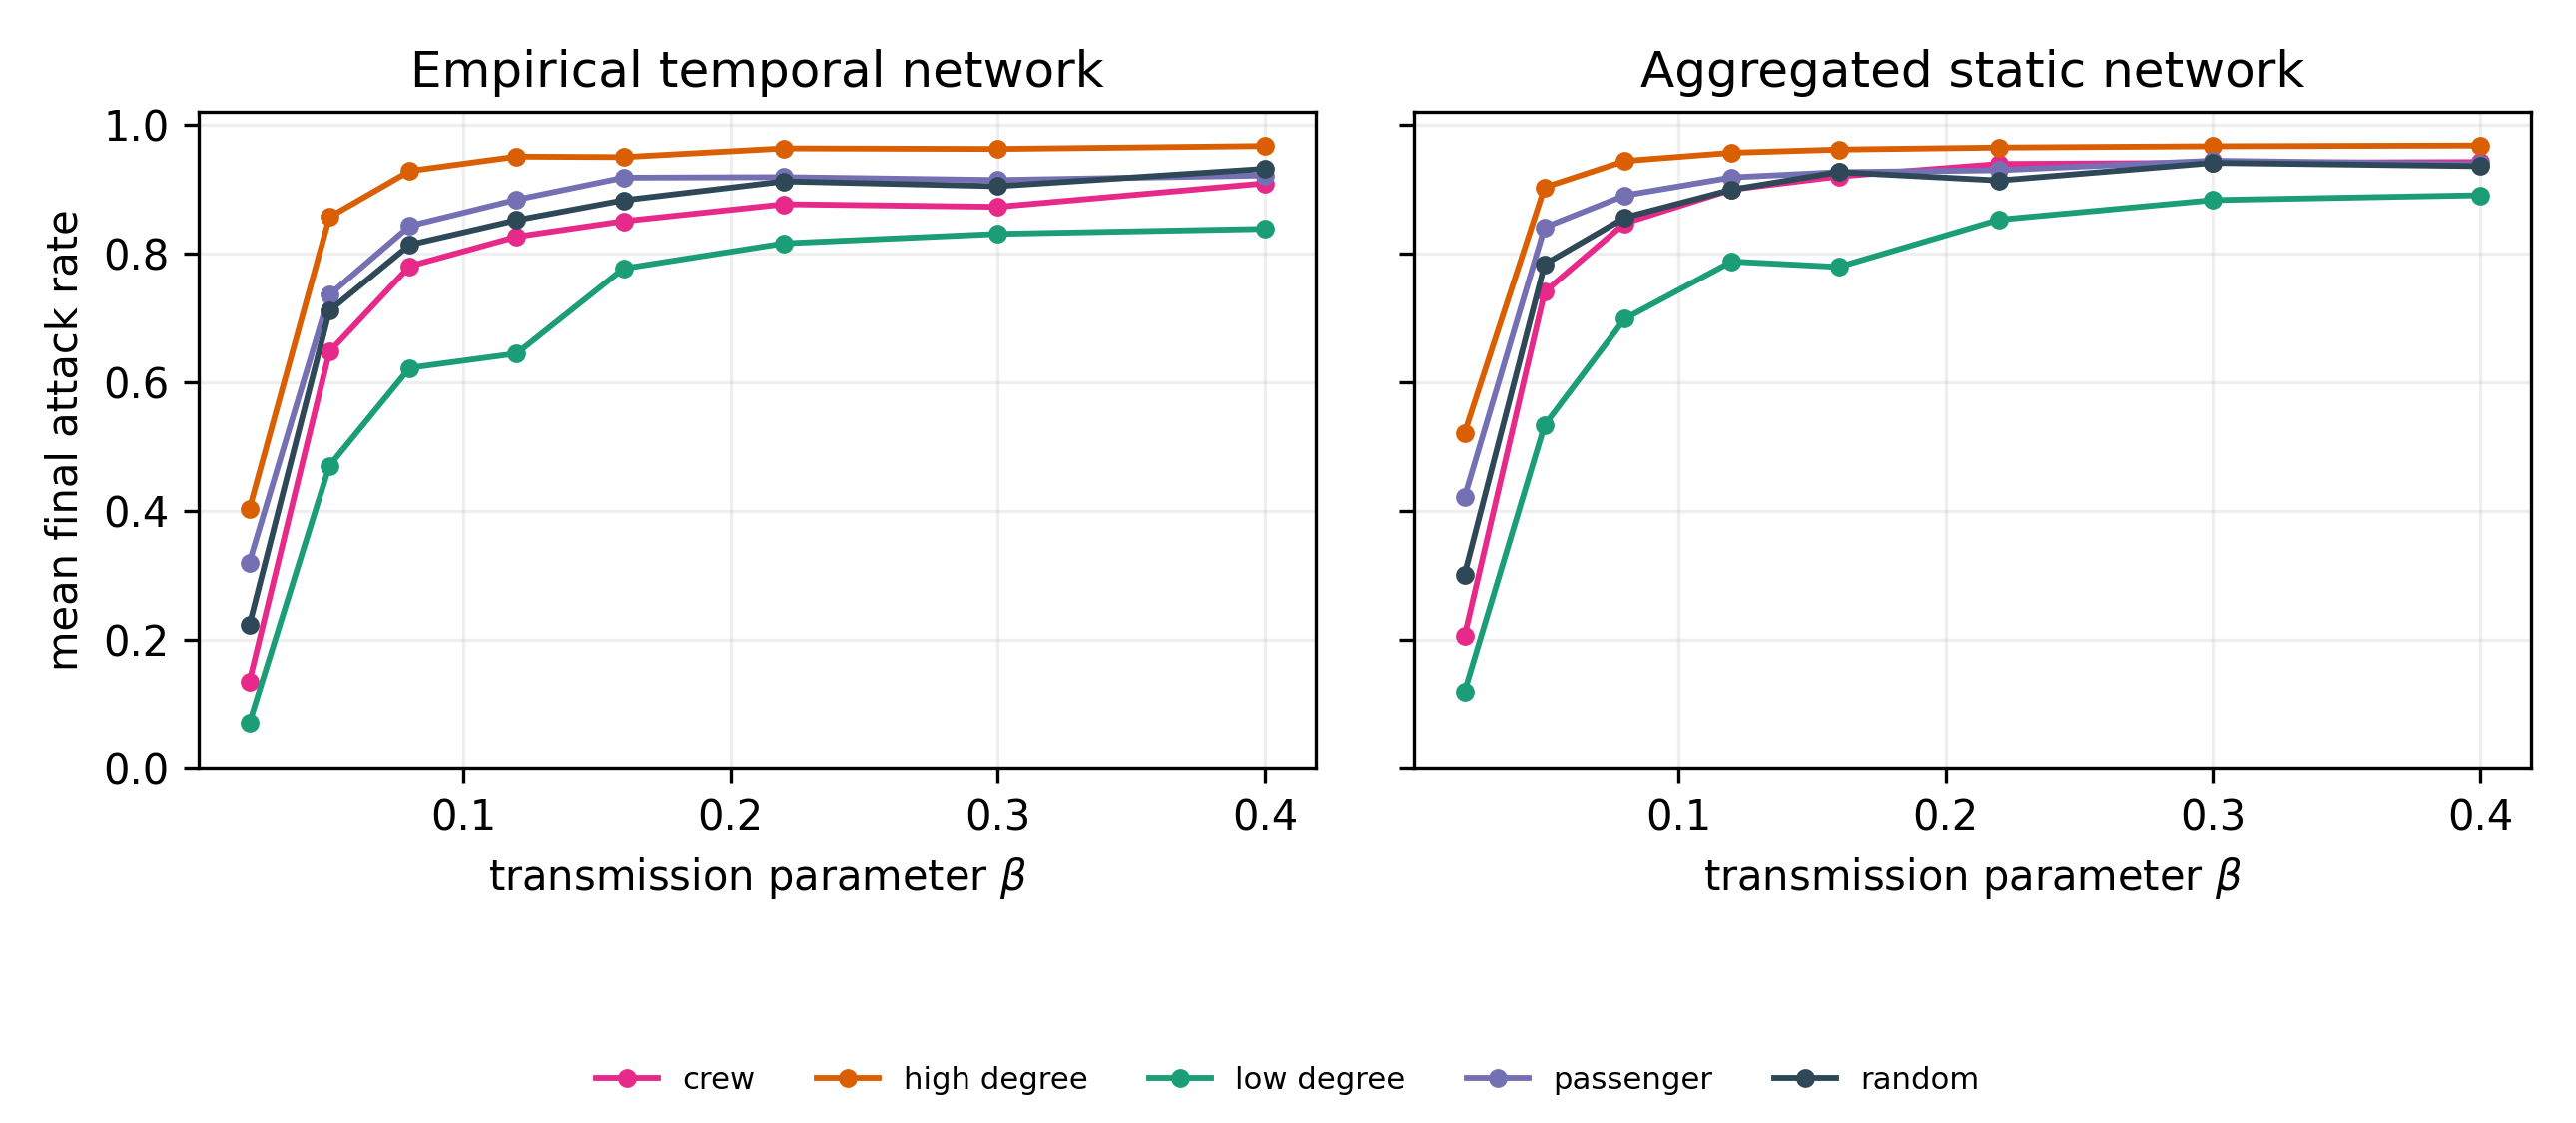
\includegraphics[width=.97\linewidth]{results/cruise_epidemic_corrected/corrected_seed_strategy_attack_rate.png}
\caption{Dependence of mean final attack rate on the initial seed-node pool.}
\label{fig:cruise-seed}
\end{figure}

The result is that, if the epidemic starts on high-degree nodes, it produces large outbreaks in both representations even for low values of $\beta$. On the other hand, initial infected low-degree nodes produce lower final attack rate. Finally, random seed nodes final attack rates are placed between crew and passanger respective attack rates.
This does not surprise because there are far more passenger than crew members in the ship, and a random sample is likely to fall more often in the passenger class rather than the crew one.\\
The static representation again gives larger outbreaks for the same seed-selection strategy, but the differences are not so high when it comes to high-degree nodes selection strategy.
